\section{Results}
\label{sec:results}

All 4,040 first-stage confirmation responses received three valid event codes, yielding
12,120 coder outputs and 32,320 majority-coded response--event observations.
The six disclosed larger-budget codes are included; the original failures are
retained. On this complete panel, pairwise positive coder agreement is
99.05--99.29\% for answer revelation, 91.38--92.52\% for reasoning elicitation,
and 96.29--98.15\% for affect acknowledgement. These are measurement diagnostics
over all arms, distinct from the repeated-generation agreement below.

\subsection{Different Defaults, Uneven Repetition (RQ1)}

On the 32 canonical source problems, the deployments differ substantially in
their action frequencies (Table~\ref{tab:default-rates}). GLM reveals an answer
in 22.3\% of responses and elicits reasoning in 96.5\%; DeepSeek and Doubao
reveal answers in every response, with elicitation below 5\%. M3 combines
both actions in 81/256 responses (31.6\%). These pooled profiles need not distinguish every
model pair: DeepSeek and Doubao have the same observed answer-revelation rate.

\begin{table}[t]
\centering\small
\begin{tabular}{lrrr}
\toprule
Deployment & Reveal & Elicit & Acknowledge \\
\midrule
MiniMax-M2.7 & 99.6 & 8.2 & 27.0 \\
MiniMax-M3 & 83.2 & 48.4 & 69.9 \\
DeepSeek-V4-Pro & 100.0 & 2.0 & 59.0 \\
Doubao-Seed-2.0-Lite & 100.0 & 4.3 & 60.9 \\
GLM-5.3 & 22.3 & 96.5 & 51.2 \\
\bottomrule
\end{tabular}
\caption{Canonical event rates (\%): 256 answers per deployment, eight per
source, on 32 sources. Events can co-occur. Abbreviated deployment names in the
text refer to these configurations, not all releases in their model families.}
\label{tab:default-rates}
\end{table}

Recurring distributions do not imply identical actions on repeated requests.
M3's elicitation agreement is only 57.8\% across 128 matched input pairs
(95\% source-bootstrap interval 50.0--66.4\%). Conversely, DeepSeek and Doubao
have 96.1\% and 91.4\% elicitation agreement but zero positive agreement:
their few positive occurrences do not recur in both requests. Perfect answer
agreement for these two deployments reflects an observed ceiling. We therefore
interpret recurrence through prevalence, agreement on presence and absence,
and prospective prediction together (Appendix~\ref{app:confirmation-details}).
Appendix~\ref{app:materials-examples} provides a same-input response set,
including a coding disagreement, to illustrate the event distinctions.

\subsection{New-Problem Transfer Under Original Wording (RQ2)}

All three model-default predictors improve over the situation-only baseline
on new sources (Appendix Figure~\ref{fig:primary-gains}). The absolute Brier reductions
are 0.09127 for revelation, 0.12970 for elicitation, and 0.01982 for
acknowledgement; all pass the six-test Holm correction. Absolute losses fall
from 0.15359 to 0.06232, 0.21873 to 0.08903, and 0.18242 to 0.16260,
respectively. Thus the identity-specific information learned before confirmation
predicts actions beyond the supplied subject and student-state context.



Adding model-specific student-state responses to model-by-subject profiles
gives a different result. Acknowledgement improves by 0.00973
(95\% interval [0.00536, 0.01395], adjusted $p=0.000192$), reducing Brier loss
from 0.16046 to 0.15072. Revelation gains only 0.00043
([-0.00037, 0.00130], $p=0.326$); elicitation changes by -0.00016
([-0.00101, 0.00073], $p=0.641$). These unresolved increments concern
the specified cues and predictor class, not every possible form of adaptation.

The training-only length/formatting competitor yields losses of 0.13861,
0.17826, and 0.17864 for the three events, exceeding the model-default losses
in each case. This descriptive comparison shows that two simple style summaries
do not reproduce the predictive result. It neither excludes richer stylistic
explanations nor identifies a causal effect of model identity.

\subsection{Prediction Under New Student Wording (RQ2)}
\label{sec:cue-results}

When students express themselves differently, the original model defaults still
help predict whether tutors give answers or invite reasoning. For acknowledgement,
the extra benefit of knowing each model's response to student cues is lost.
This benefit remains positive when we collect new replies using the original
wording during the same period. The contrast weakens an explanation based only on a general loss of predictive
value over time. Figure~\ref{fig:expression-transfer}
shows the estimates and uncertainty; Appendix Table~\ref{tab:cue-primary}
gives all six tests and Appendix~\ref{app:cue-transfer} the paired contrasts.

\begin{figure}[t]
\centering
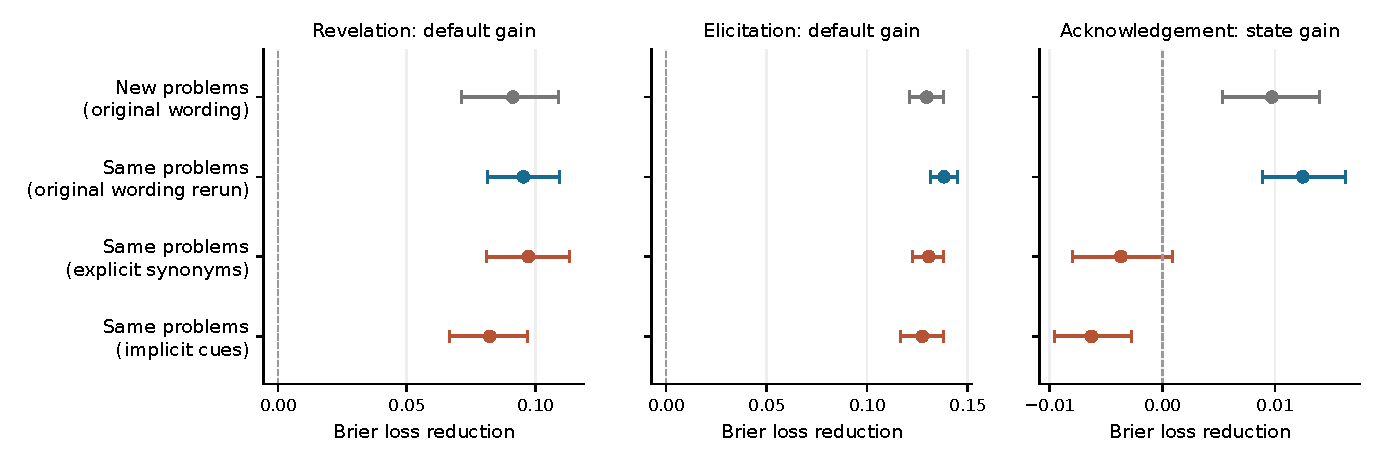
\includegraphics[width=\linewidth]{figures/expression_transfer.pdf}
\caption{Transfer depends on what is changed. The initial test uses
new problems with the original wording. The three follow-up conditions use
those same 32 problems and the earlier predictions. Default gains for giving answers and
inviting reasoning remain positive, while the state gain for acknowledgement
is no longer positive under new wording. Bars are source bootstrap 95\%
intervals conditional on frozen fits, not four independent replications or
simultaneous intervals. Horizontal scales differ by panel.}
\label{fig:expression-transfer}
\end{figure}

The acknowledgement gains have the same sign pattern when each annotator's labels
are used separately and when each generating model is left out, although some
intervals include zero. These checks reuse the same responses. The result
concerns prediction: models still acknowledge feeling or difficulty at different
rates for contrasting student cues. It does not mean that models stop responding to
student cues. The implicit condition also changes more than affect wording.

\paragraph{Alternative explanations.}
Losing an advantage over a baseline does not always mean making larger errors.
Under explicit synonyms, the cue-based predictor's own loss improves slightly,
yet it no longer outperforms the baseline. Under implicit cues, its own loss
also worsens. Further checks show that a common change in acknowledgement
frequency cannot explain the contrast, and the tested logistic recalibrations
do not restore a positive gain. These follow-up analyses narrow the explanations
without identifying a unique mechanism
(Appendices~\ref{app:cue-diagnosis}--\ref{app:cue-calibration}).

In the additional classmate control, changing a classmate's quoted feelings changes
acknowledgement rates even though the current student remains calm. Selected
examples show this can happen when the model correctly distinguishes the two
students' feelings. The contrast alone therefore does not establish confusion
about whose feelings are being expressed (Appendix~\ref{app:cue-transfer}).


\subsection{Instructions Converge on Demanded Actions (RQ3)}

The matched prompt comparison uses 16 sources and 128 answers per deployment
per arm. ASK requires eliciting a next step without stating the final answer.
All five deployments elicit reasoning in all 128 ASK responses. Revelation
falls to zero for DeepSeek, Doubao, and GLM, but remains in 9/128 M2.7 and
4/128 M3 responses. EXPLAIN instead requires a solution and final answer,
while explicitly permitting follow-up reasoning or questions. Every deployment
reveals the answer in every EXPLAIN response.

Convergence on the requested action does not eliminate all observed differences.
Under EXPLAIN, elicitation occurs in 62.5\% of GLM and 45.3\% of M3 responses,
compared with 1.6--5.5\% for the other three deployments. Since all these
responses reveal the answer, those rates also describe joint revelation and
elicitation. This permitted behavior is not an instruction violation, and the
event codes do not establish its temporal order. A single answer-versus-question
axis would hide it. Matched rates and paired prompt changes are reported in
Appendix~\ref{app:confirmation-details}.

Neutral role paraphrases place a further limit on stable-type interpretations.
For GLM, neutral B raises both revelation and acknowledgement by 15.6 percentage
points relative to the matched canonical arm. These are observed shifts, not
additional primary tests. No neutral comparison establishes population
equivalence within $\pm 0.10$ under the disclosed bounded-source check: with
16 sources its simultaneous half-width is 0.9414. This lack of precision
cannot be used as evidence for either universal stability or universal wording
sensitivity.

\subsection{Instruction Dependence in Archived Dialogue}

The archive's seven historical configurations also differ under general
scaffolding instructions: revelation ranges from 22.27--86.33\% and elicitation
from 12.11--73.44\%. Source-held-out model rates improve Brier loss by
0.04681 [0.03834, 0.05528] and 0.04193 [0.03385, 0.05011], respectively.
Under explicit probing instructions, revelation falls to 1.95--13.28\% and
elicitation concentrates at 89.84--98.83\%; model gains shrink to 0.00081
[0.00013, 0.00156] and 0.00041 [-0.00006, 0.00092].
Directly transferring the other instruction's model probabilities produces
negative revelation and elicitation gains in both directions
(Appendix~\ref{app:archive-validation}). These are descriptive, conditional
cross-fit intervals, not additional confirmatory tests.

The scaffolding gains remain positive across single coders on 254 complete
sources and all seven generator exclusions. Acknowledgement, however, occurs
in only 27/1,792 scaffolding and 25/1,792 probing replies, with positive coder
agreement of 65.55--66.67\%. Its near-zero predictive gains cannot establish
absence of affect responsiveness. Historical deployment aliases and
reconstructed requests preclude attributing cross-study rate changes solely
to context. This archive tests instruction dependence in benchmark snippets,
not learning outcomes or transfer of the original fitted predictor.

\subsection{Dependence on Measurement and Model Composition}

The first-stage default/conditional distinction persists across eight coding
panels, but its strength depends on model composition. Removing GLM reduces
default gains to 0.00394 for revelation and 0.03080 for elicitation; removing
M2.7 reduces default acknowledgement gain to 0.00175 with an interval spanning
zero. The findings therefore do not imply equally strong differences among
all deployment subsets. Two hundred training-source resamples and enumeration
of the disclosed missing confirmation votes preserve the main predictive
pattern (Appendix~\ref{app:confirmation-details}).

Content-screened matched subsets retain the predictive pattern, including a
conditional acknowledgement gain of 0.00989 [0.00510, 0.01472] after excluding
all five-model slots flagged by either reviewer. This retains 1,065 responses
on all 32 sources. However, the reviewers share only 5 of the 49 error flags,
with 18.5\% positive agreement despite passing the diagnostic controls.
Screening tests dependence on those judgments; it neither guarantees correctness
nor causally separates behavior from ability. Full rates, sensitivity ranges,
and mathematics/content subsets appear in Appendix~\ref{app:content-results}.
